% =============================================================================
\section{Squeezing by component separation}
% =============================================================================

As an example of measurement of the degree of squeezing in a real two-component \abbrev{bec} system, we will consider a recent experiment~\cite{Riedel2010}, in which multi-particle entanglement and resulting spin squeezing was achieved with the help of component-dependent potential.

The experiment essentialy consisted of the same regular Ramsey sequence as depicted in~\figref{bec-noise:visibility:sequences},~(a) performed on $1250$ \Rb{} atoms in the hyperfine state ${\ket{F=1,\, m_F=-1}}$ in a cigar-shaped trap with $f_x = f_y = 109\un{Hz}$, $f_z = 500\un{Hz}$.
The experiment started with the application of a $\pi/2$-pulse using an oscillator with the Rabi frequency $\Omega=2.1\un{kHz}$, creating an equal superposition of two hyperfine states ${\ket{F=1,\, m_F=-1}}$ and ${\ket{F=2,\, m_F=+1}}$.
The second pulse had varied length allowing a measurement of the spin along the angle $\theta$: $\hat{S}_\theta = \hat{S}_z \cos \theta - \hat{S}_y \sin \theta$ (spin tomography).

The imporant difference was an addition of the component-dependent longitudinal shift to the potential $l_x = \pm 0.26\un{\mu m}$ right after the first pulse (as described by~\eqnref{bec-noise:system:V}), persisting the whole time of the evolution until the second oscillator pulse.
This effectively reduced the component overlap and provided a way of controlling the nonlinearity and the spin squeezing according to the ``one-axis twisting Hamiltonian'' model~\cite{Kitagawa1993}.

\begin{figure}
    %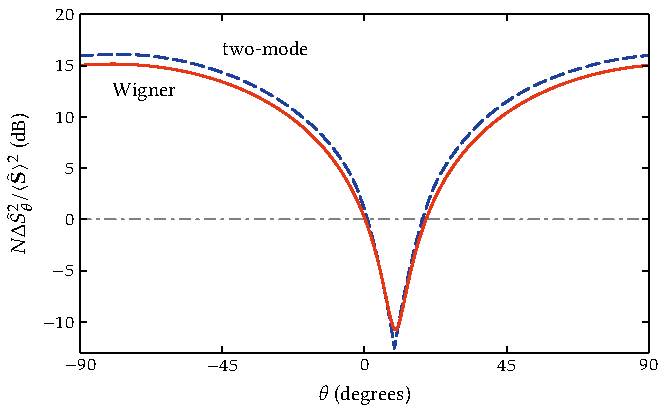
\includegraphics{figures_generated/squeezing/riedel_rotation.pdf}

    \caption{
    The dependence of the normalized variance on the rotation angle $\theta$ for
    the Wigner method (red solid line, with sampling errors marked with red dashed lines) and the two-mode variational method (dashed blue line, data taken from~\cite{Riedel2010}).
    }
    \label{fig:bec-squeezing:separation:tomography}
\end{figure}

The truncated Wigner approach is applied straightforwardly to this system and allows us to measure the degree of squeezing $xi^2$ according to the formula~\eqnref{bec-squeezing:theory:xi2}, calculating the required spin correlations using the expressions derived in \secref{bec-squeezing:theory}.
Furthermore, we can simulate the observations closer to those used in the experiment, and collect the spin tomography results, as shown in~\figref{bec-squeezing:separation:tomography}.
The maximum degree of squeezing and the corresponding rotation angle corresponds to the minimum of the graph.

The Wigner method shows good agreement with the two-mode variational method~\cite{Li2009}, which was used by the experimental team, and also includes the effect of particle losses.
The two-mode method predictions were taken from~\cite{Riedel2010} and plotted in~\figref{bec-squeezing:separation:tomography} for the sake of comparison \todo{can we do that?}.
The figure demonstrates that the predictions of the two methods for the maximum squeezing angle are nearly identical, and the predictions of the degree of squeezing are close, yet noticeable different ($-10.73\pm0.05\un{dB}$ from the Wigner method as compared with $-12.8\un{dB}$ from the two-mode method).
We believe this is caused by the Wigner method being a more systematic type of approximation with a small parameter, and consequently, more suitable for such complex calculations.

This prediction is hard to verify experimentally, as the technical noise greatly reduces the degree of squeezing (down to $-3.7\un{dB}$), moving it far from the theoretical limit.
The technical noise was not included in the simulations in this thesis, although it can be done similarly to \charef{bec-noise} (since the techincal noise in this experiment has the same nature).
On the other hand, the maximum ``unsqueezing'' (the maximums of the plot in~\figref{bec-squeezing:separation:tomography}), while being irrelevant for practical purposes, can serve as a good experimental check for the two-mode and Wigner methods, as it is much less affected by the technical noise.
The difference of $1\un{dB}$ in the maximum unsqueezing between the two methods should be possible to distinguish.

\begin{figure}
    %\includegraphics{figures_generated/squeezing/riedel_cloud_yz.pdf}

    \caption{
    Reconstructed probability distribution for the value of the spin vector projected on $y,z$ plane (a) and spin noise tomography (b).
    The variance $\Delta^2 \hat{S}_\theta$ is connected to the width of the distribution $d_\theta$ in direction $\theta$
    (blue line between two arrows in panel (a)) as
    $2 \sqrt{\Delta^2 \hat{S}_\theta} = d_\theta$.}
    \label{fig:bec-squeezing:separation:cloud-yz}
\end{figure}

We can go further and reconstruct the spin noise distribution using the per-path values of the total spin components, as explained in the end of \secref{bec-squeezing:theory}.
The uncertainty of the total spin in the orthogonal plane is shown in~\figref{bec-squeezing:separation:cloud-yz}.
The shape of the cloud is similar to the one obtained experimentally~\cite{Riedel2010}, and it also serves as a good illustration of the physical meaning of the maximum degree of squeezing and the corresponding rotation angle.
The shot noise limit of $\sqrt{N}$ corresponding to the initial number of atoms is also plotted as a red dash-dotted circle.

It is interesting to look at all three projections of the cloud, shown in~\figref{bec-squeezing:separation:cloud-yz}.
It is clearly seen that indeed the direction used to measure the squeezing in the experiment is indeed the best one, and the cloud is much wider in other directions.
